\documentclass{standalone}
\usepackage{tikz}
\usetikzlibrary{shapes,arrows,decorations.pathreplacing}
\tikzset{font=\footnotesize}
% Colour defs
\definecolor{myGreen}{HTML}{7fc97f}
\definecolor{myPurple}{HTML}{beaed4}
\begin{document}
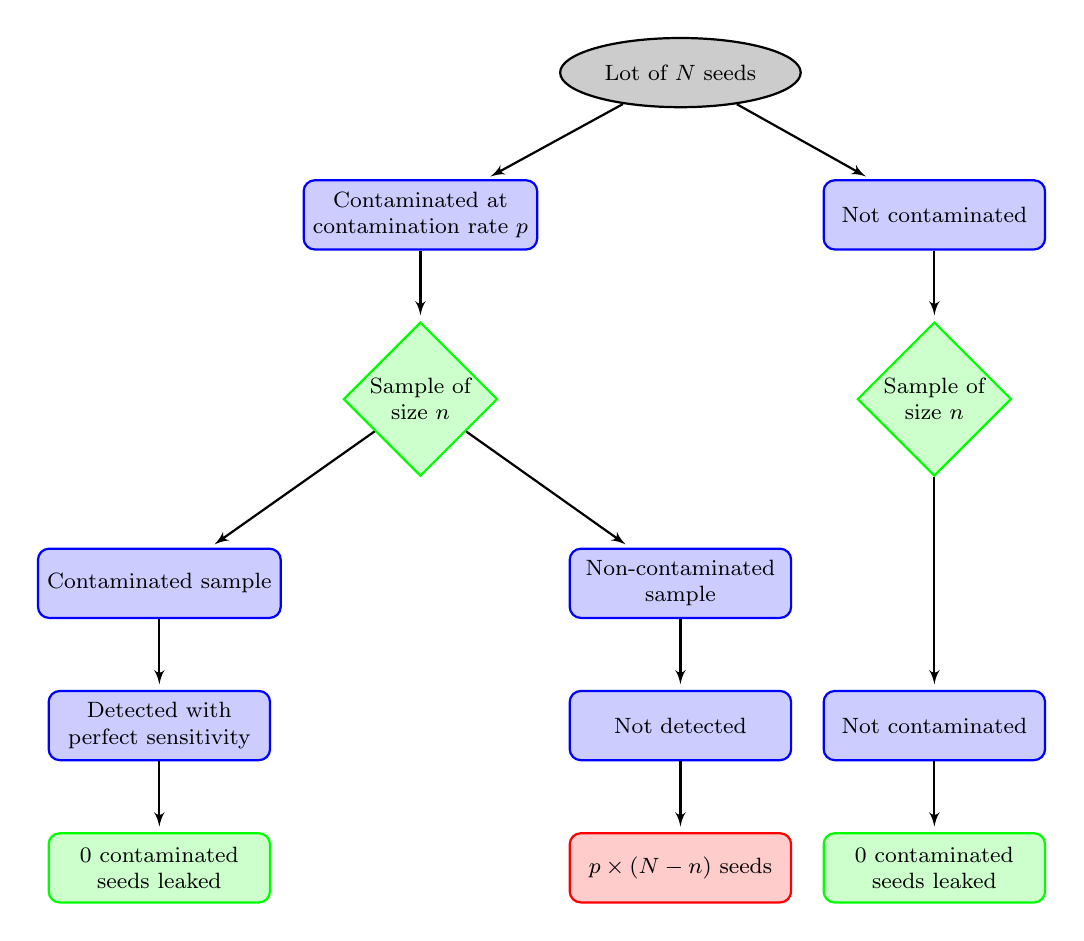
\begin{tikzpicture}
  [auto, every node/.style={transform shape, minimum width=3.5em},
  decision/.style={diamond, draw=blue, thick, fill=blue!20,align=flush center,inner sep=1pt},
  gdecision/.style={diamond, draw=green, thick, fill=green!20,align=flush center,inner sep=1pt},
  bdecision/.style={diamond, draw=brown, thick, fill=brown!20,align=flush center,inner sep=1pt},
  block/.style ={rectangle, draw=blue, thick, fill=blue!20,align=center, rounded corners, minimum width = 8em, minimum height = 2.5em},
  rblock/.style ={rectangle, draw=red, thick, fill=red!20,align=center, rounded corners, minimum width = 8em, minimum height = 2.5em},
  gblock/.style ={rectangle, draw=green, thick, fill=green!20,align=center, rounded corners, minimum width = 8em, minimum height = 2.5em},
  line/.style ={draw, thick, -latex',shorten >=2pt},
  cloud/.style ={draw=black, thick, ellipse,fill=black!20,
    minimum height=2.5em,minimum width = 8em}]
  \matrix [column sep=0.75em, row sep=9mm] {
    % row 1
    & & \node [cloud] (lot){Lot of $N$ seeds}; & \\
    % row 2
    & \node [block] (contaminated){Contaminated at\\contamination rate $p$}; & & \node [block] (notInfected){Not contaminated}; \\
    % row 3
    & \node [gdecision] (sample1){Sample of\\size $n$}; & & \node [gdecision] (sample2){Sample of\\size $n$}; \\
    % row 4
    \node [block] (contaminatedSample){Contaminated sample}; & & \node [block] (nonInfectedSample){Non-contaminated\\sample}; & \\
    % row 5
    \node [block] (detected){Detected with\\perfect sensitivity}; & & \node [block] (infNotDet){Not detected}; & \node [block] (notInfNotDet){Not contaminated}; \\
    % row 6
    \node [gblock] (detected1){0 contaminated\\seeds leaked}; & & \node [rblock] (infNotDet1){$p \times (N - n)$ seeds}; & \node [gblock] (notInfNotDet1){0 contaminated\\seeds leaked}; \\
  };

  \begin{scope}[every path/.style=line]
    \path (lot) -- (contaminated);
    \path (lot) -- (notInfected);
    \path (contaminated) -- (sample1);
    \path (sample1) -- (contaminatedSample);
    \path (sample1) -- (nonInfectedSample);
    \path (notInfected) -- (sample2);
    \path (sample2) -- (notInfNotDet);
    \path (contaminatedSample) -- (detected);
    \path (nonInfectedSample) -- (infNotDet);
    \path (detected) -- (detected1);
    \path (infNotDet) -- (infNotDet1);
    \path (notInfNotDet) -- (notInfNotDet1);
 \end{scope}
\end{tikzpicture}
\end{document}

%%% Local Variables:
%%% mode: latex
%%% TeX-master: t
%%% End:
